% Please use the skeleton file you have received in the
% invitation-to-submit email, where your data are already
% filled in. Otherwise please make sure you insert your
% data according to the instructions in PoSauthmanual.pdf
\documentclass[a4paper]{PoS}

\usepackage{amsmath}

\title{Measurement of top quark properties at CMS}

\ShortTitle{Top quark properties}

\author{\speaker{J\'onatan Piedra}\thanks{For the CMS Collaboration.}\\
        Instituto de F\'isica de Cantabria (CSIC-UC)\\
        E-mail: \email{piedra@cern.ch}}

%\author{Another Author\\
%        Affiliation\\
%        E-mail: \email{...}}

\abstract{
% W polarization
% Top quark couplings
% ttV
% R=BR(t->Wb)/BR(t->Wq)
Measurements of top quark properties in top quark decays are presented,
using data collected by the CMS experiment during the years 2011 and 2012. The
polarization of W bosons in top quark decays is measured. The W boson helicity
fractions and angular asymmetries are extracted, and limits on anomalous
contributions to the Wtb vertex are determined. Furthermore, searches for
flavor changing neutral currents in top quark decays are presented. The flavor
contents in top quark pair events are measured using the fraction of top quarks
decaying into a W boson and a b quark relative to all top quark decays,
$R=BR({\rm t} \to {\rm Wb})/BR({\rm t} \to {\rm Wq})$, and the result is used to
determine the CKM matrix element $V_{\rm tb}$ as well as the width of the top quark
resonance.
}

\FullConference{The European Physical Society Conference on High Energy Physics\\
		22--29 July 2015\\
		Vienna, Austria}


\begin{document}

%~~~~~~~~~~~~~~~~~~~~~~~~~~~~~~~~~~~~~~~~~~~~~~~~~~~~~~~~~~~~~~~~~~~~~~~~~~~~~~~
\section{The CMS detector}
%~~~~~~~~~~~~~~~~~~~~~~~~~~~~~~~~~~~~~~~~~~~~~~~~~~~~~~~~~~~~~~~~~~~~~~~~~~~~~~~

% As in PRL 112, 171802 (2014)
The central feature of the CMS apparatus is a superconducting solenoid, which
provides an axial magnetic field of 3.8~T. Within the field volume there are a
silicon pixel and strip tracker, a lead tungstate crystal electromagnetic
calorimeter, and a brass or scintillator hadron calorimeter. Charged-particle
trajectories are measured by the tracker, covering $0 \leq \phi \leq 2\pi$ in
azimuth and $|\eta| < 2.5$ in pseudorapidity, where $\eta$ is defined as
$-\ln\left[\tan(\theta/2)\right]$, and $\theta$ is the polar angle of
the trajectory of the particle with respect to the counterclockwise proton beam
direction. Muons are identified and measured in gas-ionization detectors embedded
in the steel flux return yoke outside the solenoid. A more detailed description
of CMS detector can be found in Ref.~\cite{cms}.


%~~~~~~~~~~~~~~~~~~~~~~~~~~~~~~~~~~~~~~~~~~~~~~~~~~~~~~~~~~~~~~~~~~~~~~~~~~~~~~~
\section{W polarization}
%~~~~~~~~~~~~~~~~~~~~~~~~~~~~~~~~~~~~~~~~~~~~~~~~~~~~~~~~~~~~~~~~~~~~~~~~~~~~~~~

Top quarks decay almost exclusively into a b quark and a W boson via the
electroweak interaction. Due to its large mass, the top quark decays before
hadronizing and therefore it provides the possibility to study the Lorentz
structure and coupling of the Wtb vertex. In particular, the measurement of the
W boson polarization in the top quark decays allows to probe the Wtb structure
and to search for possible extentions of the standard model (SM)~\cite{Wtb}. In
general, W bosons in the top quark decays can be produced in three states of
left-handed, right-handed, and longitudinal helicity.
Defining $\Gamma_{L,R,0}$ as the partial widths of the top quark decaying into
left-handed, right-handed, and longitudinal W boson helicities, the helicity
fractions are given by $F_{L,R,0}$ and satisfy $F_R + F_L + F_0 = 1$. Including
the next-to-next-to-leading-order (NNLO) QCD and electroweak corrections,
the W boson helicity fractions are
calculated to be $F_R = 0.0017 \pm 0.0001$, $F_0 = 0.687 \pm 0.005$, and
$F_L = 0.311 \pm 0.005$~\cite{nnlo-helicity}. The W boson helicity fractions can
be measured using the angular distributions of the top quark decay products. The
angle $\theta_{\ell}^{*}$ is defined as the angle between the 3-momentum of the
charged lepton in the W boson rest frame and the momentum of the W boson in the
top quark rest frame. The angular distribution of $\cos(\theta_{\ell}^{*})$ is
parametrized as~\cite{theta-parametrization}:
%
\begin{equation*}
\frac{1}{\Gamma}\frac{d\Gamma}{d~\cos\theta_{\ell}^*} =
\frac{3}{8}\left(1 - \cos\theta_{\ell}^*\right)^2F_L +
\frac{3}{8}\left(1 + \cos\theta_{\ell}^*\right)^2F_R +
\frac{3}{4}\sin^2\theta_{\ell}^*F_0.
\end{equation*}

In this analysis~\cite{TOP-14-017}, W boson helicity fractions are measured from
a sample of tt events with two leptons in the final state.
The method adopted for this measurement is the same as the one already used in tt
semileptonic~\cite{semileptonic-helicity-1, semileptonic-helicity-2} and dileptonic
final states~\cite{dileptonic-helicity}, and in single top quark
events~\cite{single-top-helicity} at 7 and 8~TeV by the CMS experiment.
The  analysed data sample used in this analysis corresponds to an integrated luminosity
of $19.7~{\rm fb}^{-1}$.
Events are required to contain two charged and isolated leptons with opposite sign, missing
transverse energy, and at least two b tagged jets.
The tt system kinematics can be determined using the W boson and top quark mass constraints.
By applying six kinematic constraints on the kinematics of the produced particles from top
decays, a set of solutions for neutrino and antineutrino momenta are found.
In order to extract the W boson helicity fractions, a reweighting technique is used.
It considers any arbitrary configuration of the W boson helicity fractions and the
effects of the limited experimental
resolution at the same time. The $\cos\theta_{\ell}^*$ distribution, which is used to
perform the measurement, is presented in Fig.~\ref{fig:CMS-TOP-014-017} (left).
The result from the fit is shown in Fig.~\ref{fig:CMS-TOP-014-017} (right).
The measured W boson helicity fractions are $F_L = 0.329 \pm 0.029$, $F_0 = 0.653 \pm 0.026$,
and $F_R = 0.018 \pm 0.027$.  These results are in agreement with the SM predictions at
NNLO within $2\sigma$ uncertainties.

\begin{figure}
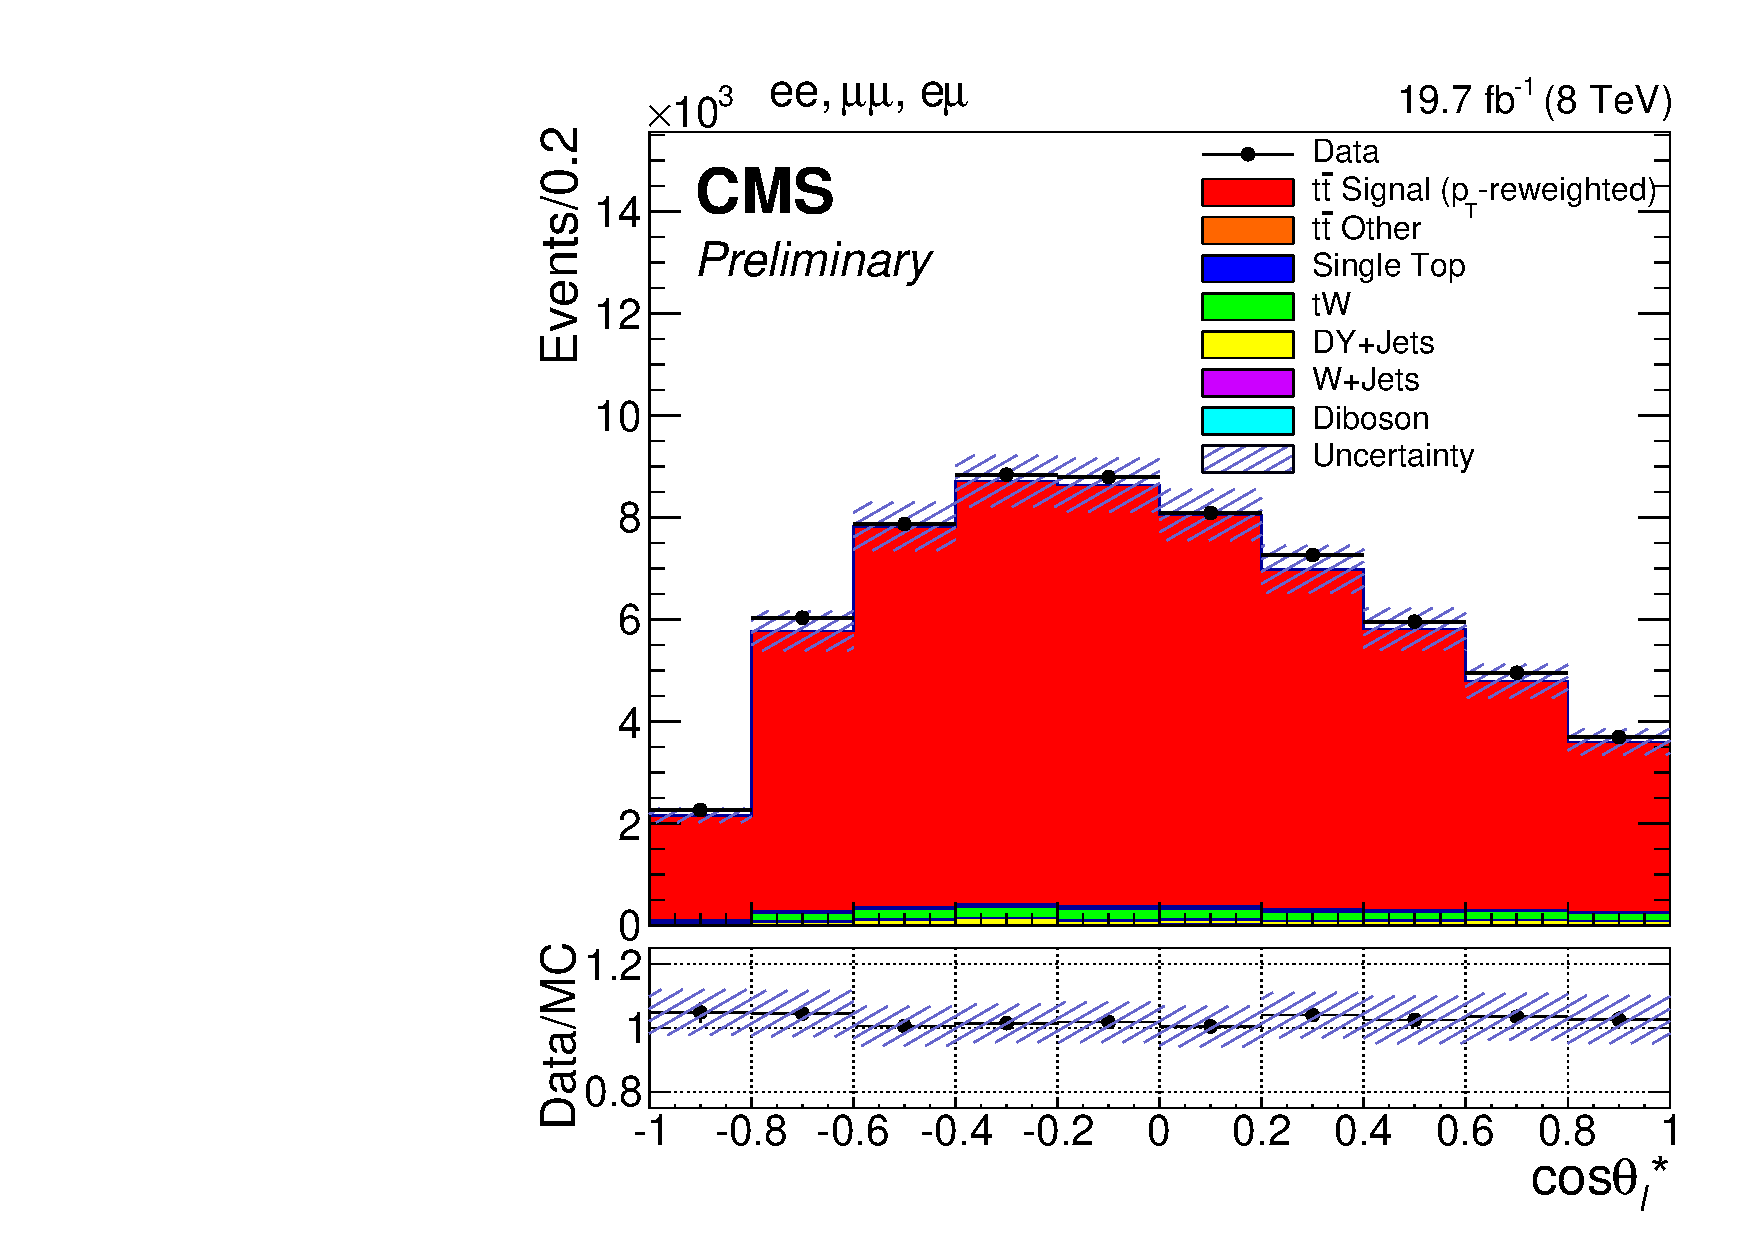
\includegraphics[width=.40\textwidth]{figures/CMS-TOP-14-017_cos_theta}
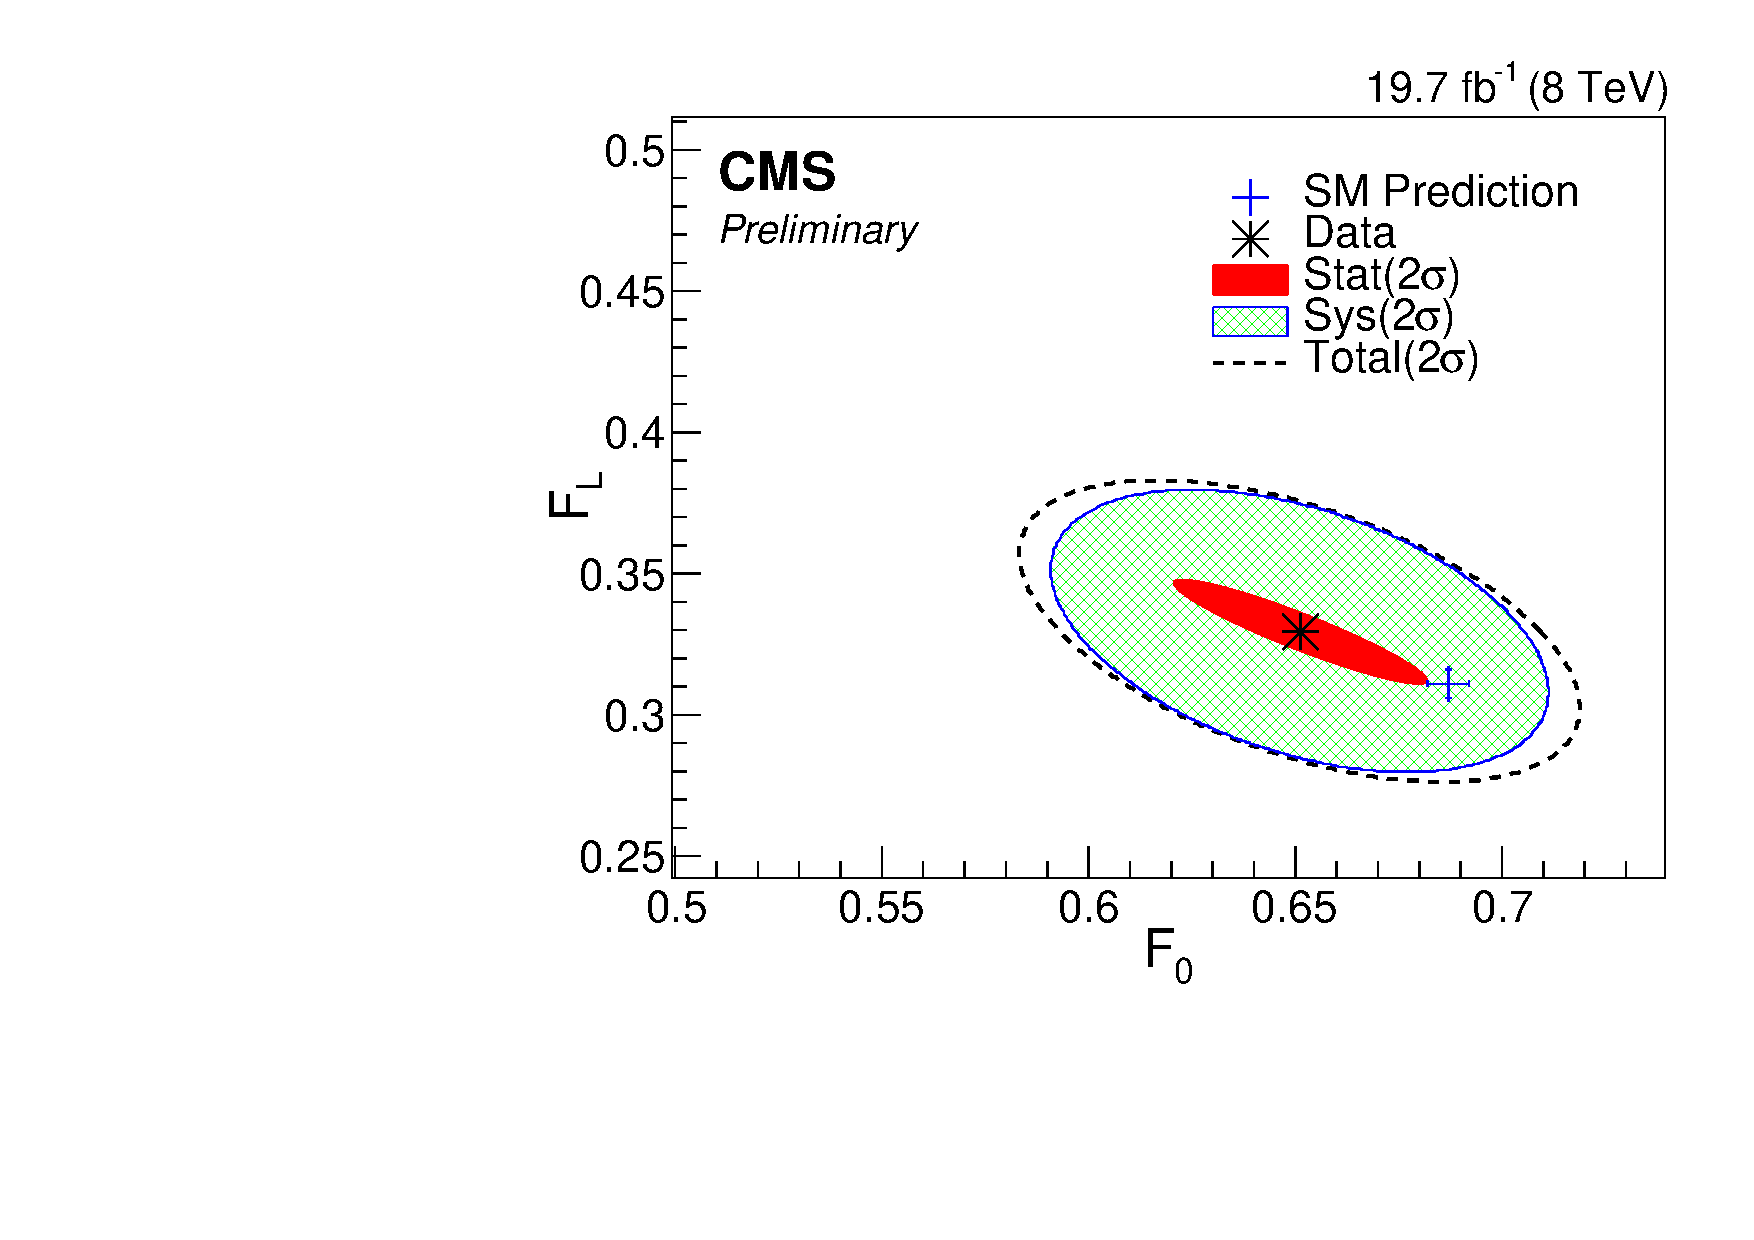
\includegraphics[width=.50\textwidth]{figures/CMS-TOP-14-017_contour_2sigma}
\caption{(Left) Distribution of $\cos\theta^*_{\ell}$ for the ee, $\mu\mu$, and e$\mu$
  channels summed. The ratio of the number of events in data to the total number
  of events from simulation is shown in the lower panel. (Right) The 95\% region
  in the ($F_0$, $F_L$) plane obtained from the fit to data. The measured and
  theoretical values of the W boson helicity fractions are shown as well.}
\label{fig:CMS-TOP-014-017}
\end{figure}


%~~~~~~~~~~~~~~~~~~~~~~~~~~~~~~~~~~~~~~~~~~~~~~~~~~~~~~~~~~~~~~~~~~~~~~~~~~~~~~~
\section{Top quark couplings}
%~~~~~~~~~~~~~~~~~~~~~~~~~~~~~~~~~~~~~~~~~~~~~~~~~~~~~~~~~~~~~~~~~~~~~~~~~~~~~~~

Within the SM, the flavor-changing neutral current (FCNC) decay of the top quark
to a Z boson and a light up-type quark (u or c), is suppressed by the GIM mechanism,
occurring only at the quantum loop level, with a branching fraction
${\cal B}({\rm t \to Zq})$ at ${\cal O}(10^{-14})$. The detection of FCNC
${\rm t \to Zq}$ decays at a higher-than-expected rate would thus be clear evidence
for physics beyond the SM.
This search~\cite{CMS_tZq_8TeV} is performed by looking for tt events where one top
quark decays into Zq and the other decays into Wb, with both vector bosons decaying
leptonically.
Events with two opposite sign, same flavor, isolated leptons, consistent with a Z boson
decay, and one extra charged lepton, are selected. Neutrinos from W boson decays escape
detection, thus we require the missing $E_{T}$ to be larger than 30~GeV.
To reduce the background from diboson events
we require at least two jets, and exactly one of these jets should be tagged
as a b quark jet.
The invariant mass of the W boson and the b tagged jet, $m_{\rm Wb}$, is required to be
within 35~GeV of the top quark mass. A non-b jet is combined with the Z candidate to form
a second top quark candidate. By examining all possible pairings, the top quark candidate
which has the largest separation in azimuthal angle to the first top quark is selected,
and the reconstructed top quark mass, $m_{\rm Zj}$, is required to be within 25 GeV of the
assumed value of 172.5~GeV. Fig.~\ref{fig:CMS-TOP-12-037} shows the comparison of the
$m_{\rm Zj}$ and $m_{\rm Wb}$ distributions in data and simulation.
After applying all the criteria $3.1 \pm 1.1$ events are expected from SM background
processes and 1 event is observed in data. A 95\%  C.L. upper limit on the branching
fraction of the ${\rm t \to Zq}$ decay  is  determined  using  the  modified frequentist
approach. Combining this result with a previous search corresponding to an integrated
luminosity of $5~{\rm fb^{-1}}$ at $\sqrt{s} = 7~{\rm TeV}$, excludes a
${\rm t \to Zq}$ branching fraction greater than 0.05\% at a confidence level
of 95\%.

\begin{figure}
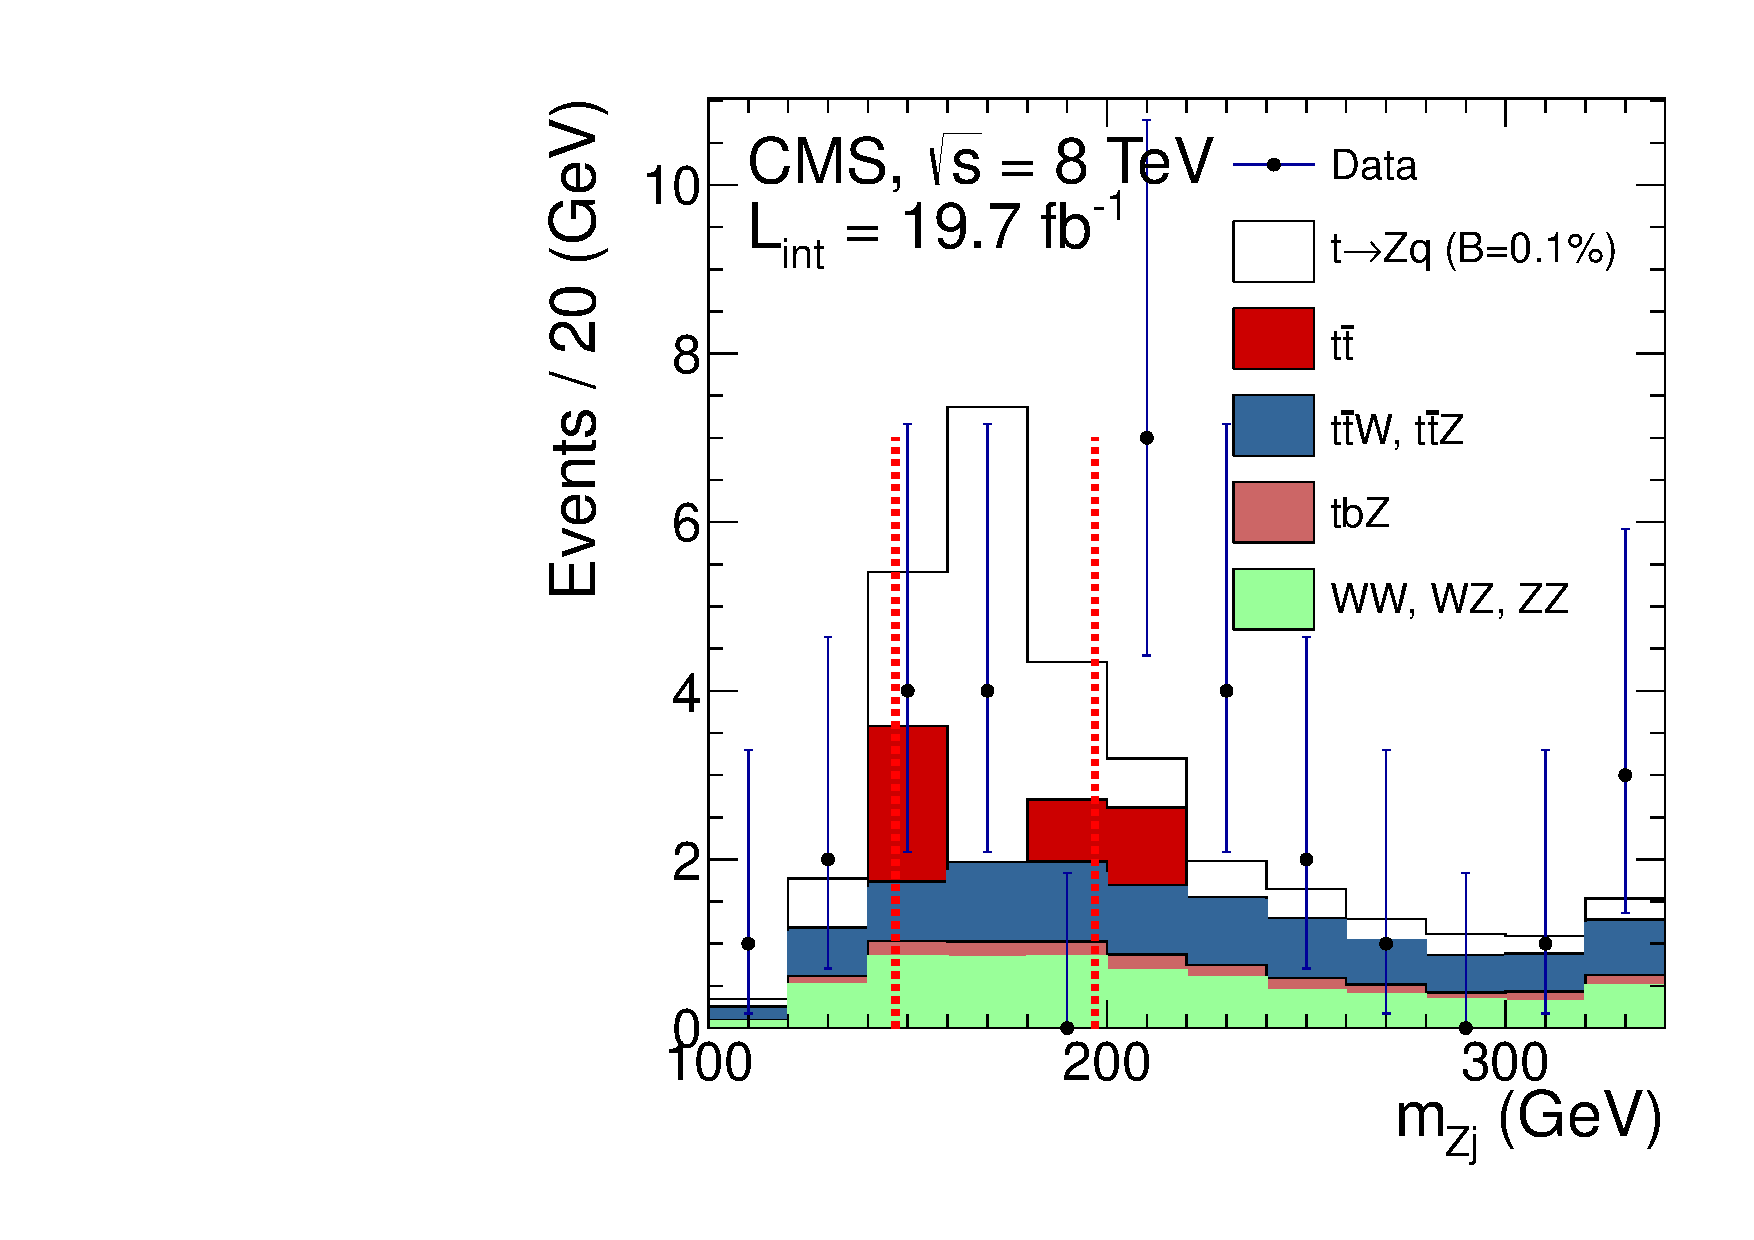
\includegraphics[width=.45\textwidth]{figures/CMS-TOP-12-037_Figure_002-a}
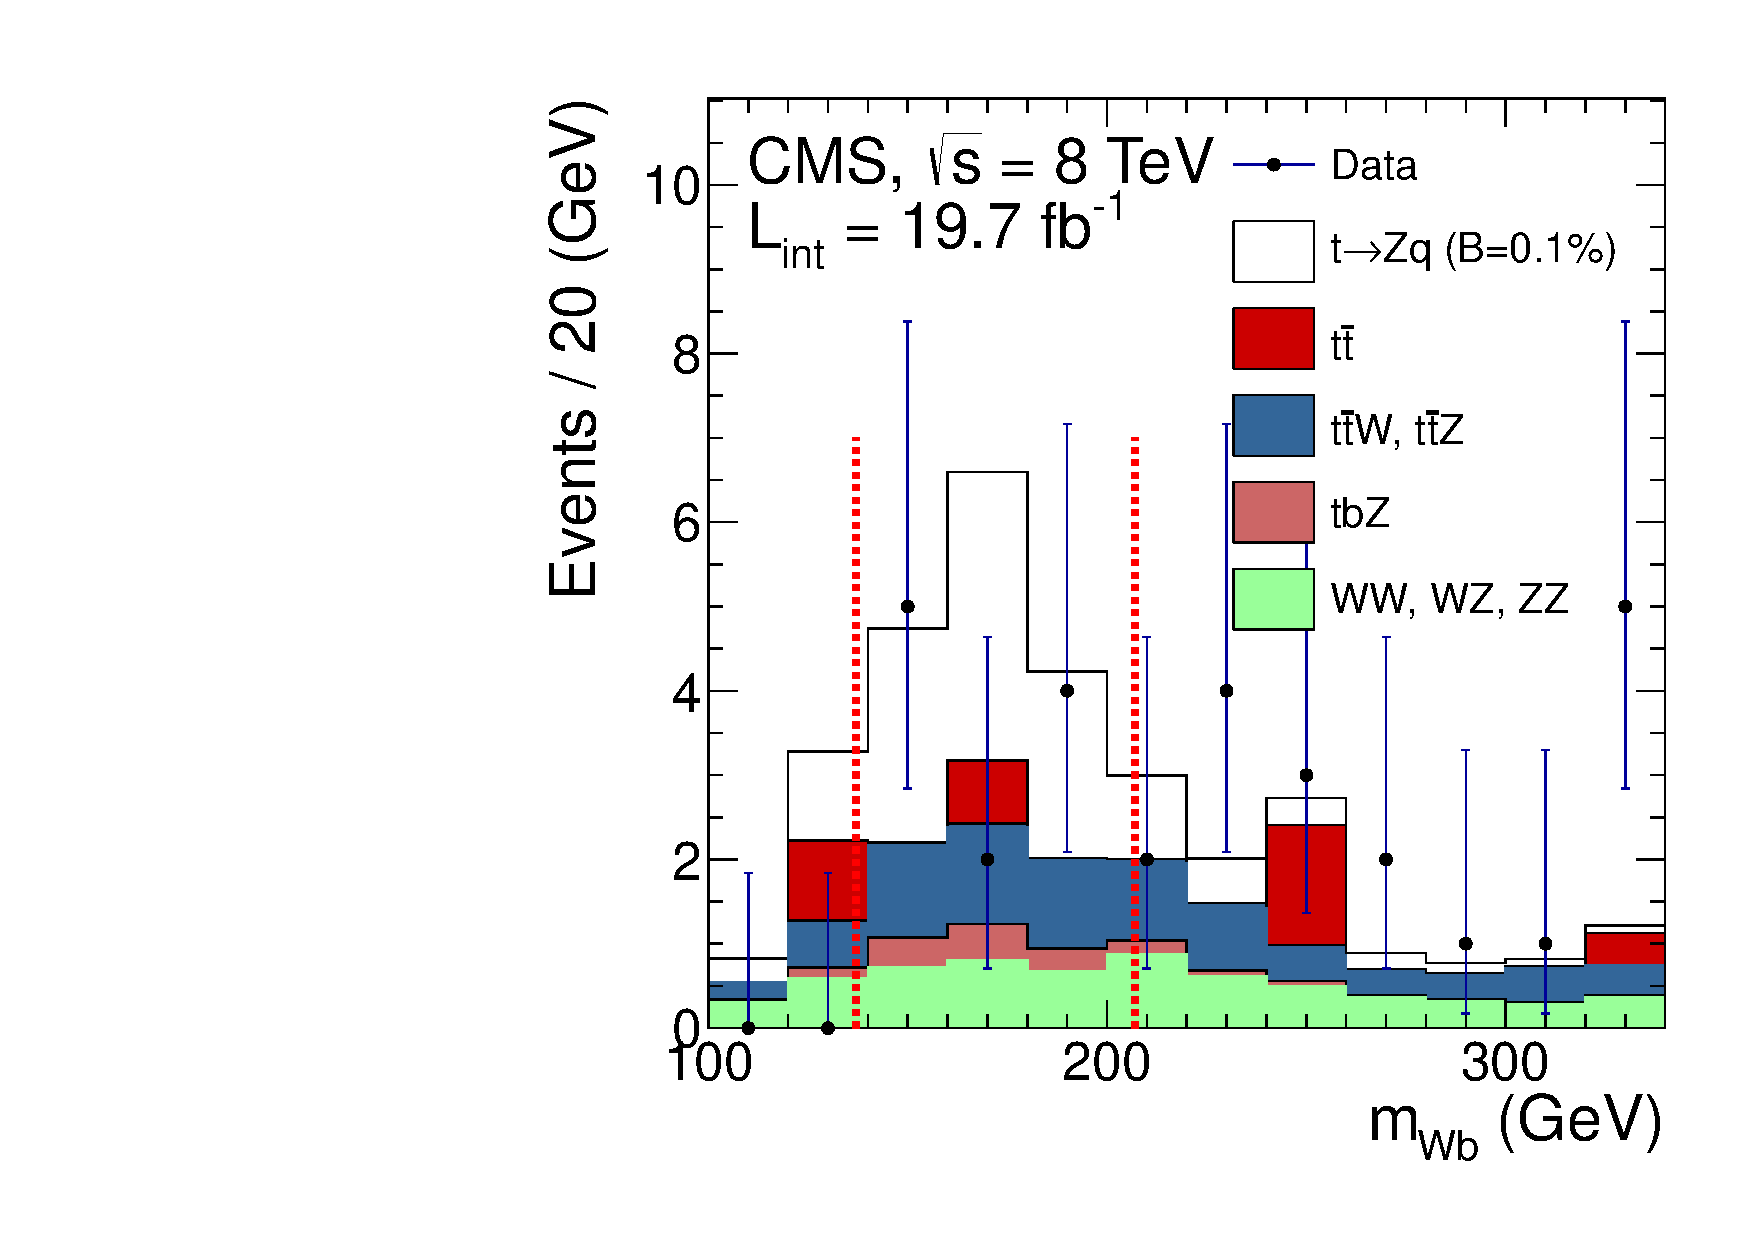
\includegraphics[width=.45\textwidth]{figures/CMS-TOP-12-037_Figure_002-b}
\caption{Comparison between data and simulated events of the $m_{\rm Zj}$ (left)
and $m_{\rm Wb}$ (right) distributions after the event selection prior to the
top quark mass requirements, which are shown as the dotted vertical lines. The
data are represented by the points with error bars and the open histogram is the
expected signal. The stacked solid histograms represent the dominant backgrounds.
The last bin in each of the two plots contains all the overflow events.}
\label{fig:CMS-TOP-12-037}
\end{figure}


%~~~~~~~~~~~~~~~~~~~~~~~~~~~~~~~~~~~~~~~~~~~~~~~~~~~~~~~~~~~~~~~~~~~~~~~~~~~~~~~
\section{Top quark pair production in association with a W or Z boson}
%~~~~~~~~~~~~~~~~~~~~~~~~~~~~~~~~~~~~~~~~~~~~~~~~~~~~~~~~~~~~~~~~~~~~~~~~~~~~~~~

The ttZ production cross section provides the most accessible direct measurement
of the top quark coupling to the Z boson. Both $\sigma({\rm ttW})$ and
$\sigma({\rm ttZ})$ would be altered in a variety of new physics models that can
be parameterized by dimension-six operators added to the standard model Lagrangian.
We present~\cite{TOP-14-021} the first measurements of the ttW and ttZ cross
sections using full event reconstruction techniques. We target events in which the
associated W boson decays to a charged lepton and a neutrino or the Z boson decays
to two charged leptons.
Events for this analysis are divided into five mutually exclusive channels.
The opposite-sign dilepton channel targets ttZ events
where the Z boson decays into an opposite sign pair of electrons or muons, and the tt system
decays hadronically.
The same sign dilepton channel selects ttW events in which the associated W boson, and the
W boson of the same charge from the tt system, each decay to a lepton and a neutrino, and
the remaining W boson decays to quarks.
The three lepton ttW channel targets events in which both the associated W and the pair of W
bosons from the tt pair decay leptonically. Furthermore, no same flavor opposite sign pair
of leptons can have a mass within 10 GeV of the Z boson mass.
The three lepton ttZ channel selects events in which the Z boson decays to a pair of electrons
or muons,  and one W boson from the tt system decays to a charged lepton and a neutrino,
with the remaining W boson decaying to quarks.  The selection is identical to the three lepton
ttW channel, except that at least one same flavor opposite sign pair of leptons must have an
invariant mass within 10 GeV of the Z boson mass.
Events with four leptons come from ttZ decays in which the Z boson and both W bosons from
the tt decay produce electrons or muons.

In each channel we attempt a full or partial reconstruction of the ttW or ttZ system with a linear
discriminant that matches leptons and jets to their parent particles using mass, charge, and b
tagging information. Additional kinematic variables from leptons and jets are combined with output
from the linear discriminant in a multivariate analysis that is used to make the final measurement
of the ttW and ttZ cross sections.
We perform separate one-dimensional fits for the ttW and ttZ cross sections using the relevant
channels for each process. The fit for each cross section is performed with the other cross section
set to the standard model (SM) value and uncertainty from theory.
The combined ttW cross section measurement in same sign and three lepton events is
$\sigma({\rm ttW}) = 382^{+117}_{-102}$~fb, corresponding to a 4.8$\sigma$ deviation from
the background-only hypothesis, where a significance of 3.5$\sigma$ was expected in
the standard model. Combining opposite sign, three lepton, and four lepton channels, the
ttZ cross section is measured to be
$\sigma({\rm ttZ}) = 242^{+65}_{-55}$~fb, an observation with a significance of 6.4$\sigma$
from the background-only hypothesis and in agreement with the standard model expectation.

Direct measurement of the ttZ and ttW cross sections can be applied to searches for new physics
(NP) within the framework of an effective field theory. The effects of new particles or
interactions can be captured in a model-independent way by supplementing the SM Lagrangian with
higher dimensional operators involving SM fields. To  study  the  effects  of  NP  on  the  ttW
and  ttZ  processes,  we  compute
cross sections as a function of the Wilson coefficients. Cross sections were computed for the
production of tt, a Higgs boson, ttZ, and ttW, sampling 20 points for each Wilson coefficient.
For each sampled point, all other Wilson coefficients were fixed at zero. From this survey,
we select five operators as of particular interest because they have a small effect on
inclusive Higgs boson and tt production, and a large effect on ttZ, ttW, or both. We have placed
limits on these five dimension-six operators:
${\bar{c}}_{uB}$,
${\bar{c}}'_{HQ}$,
${\bar{c}}_{HQ}$,
${\bar{c}}_{Hu}$,
and ${\bar{c}}_{3W}$.
Two of them are shown, for illustration, in
Fig.~\ref{fig:CMS-TOP-14-021}. All of the measured values are compatible with the
standard model predictions, within uncertainties.

\begin{figure}
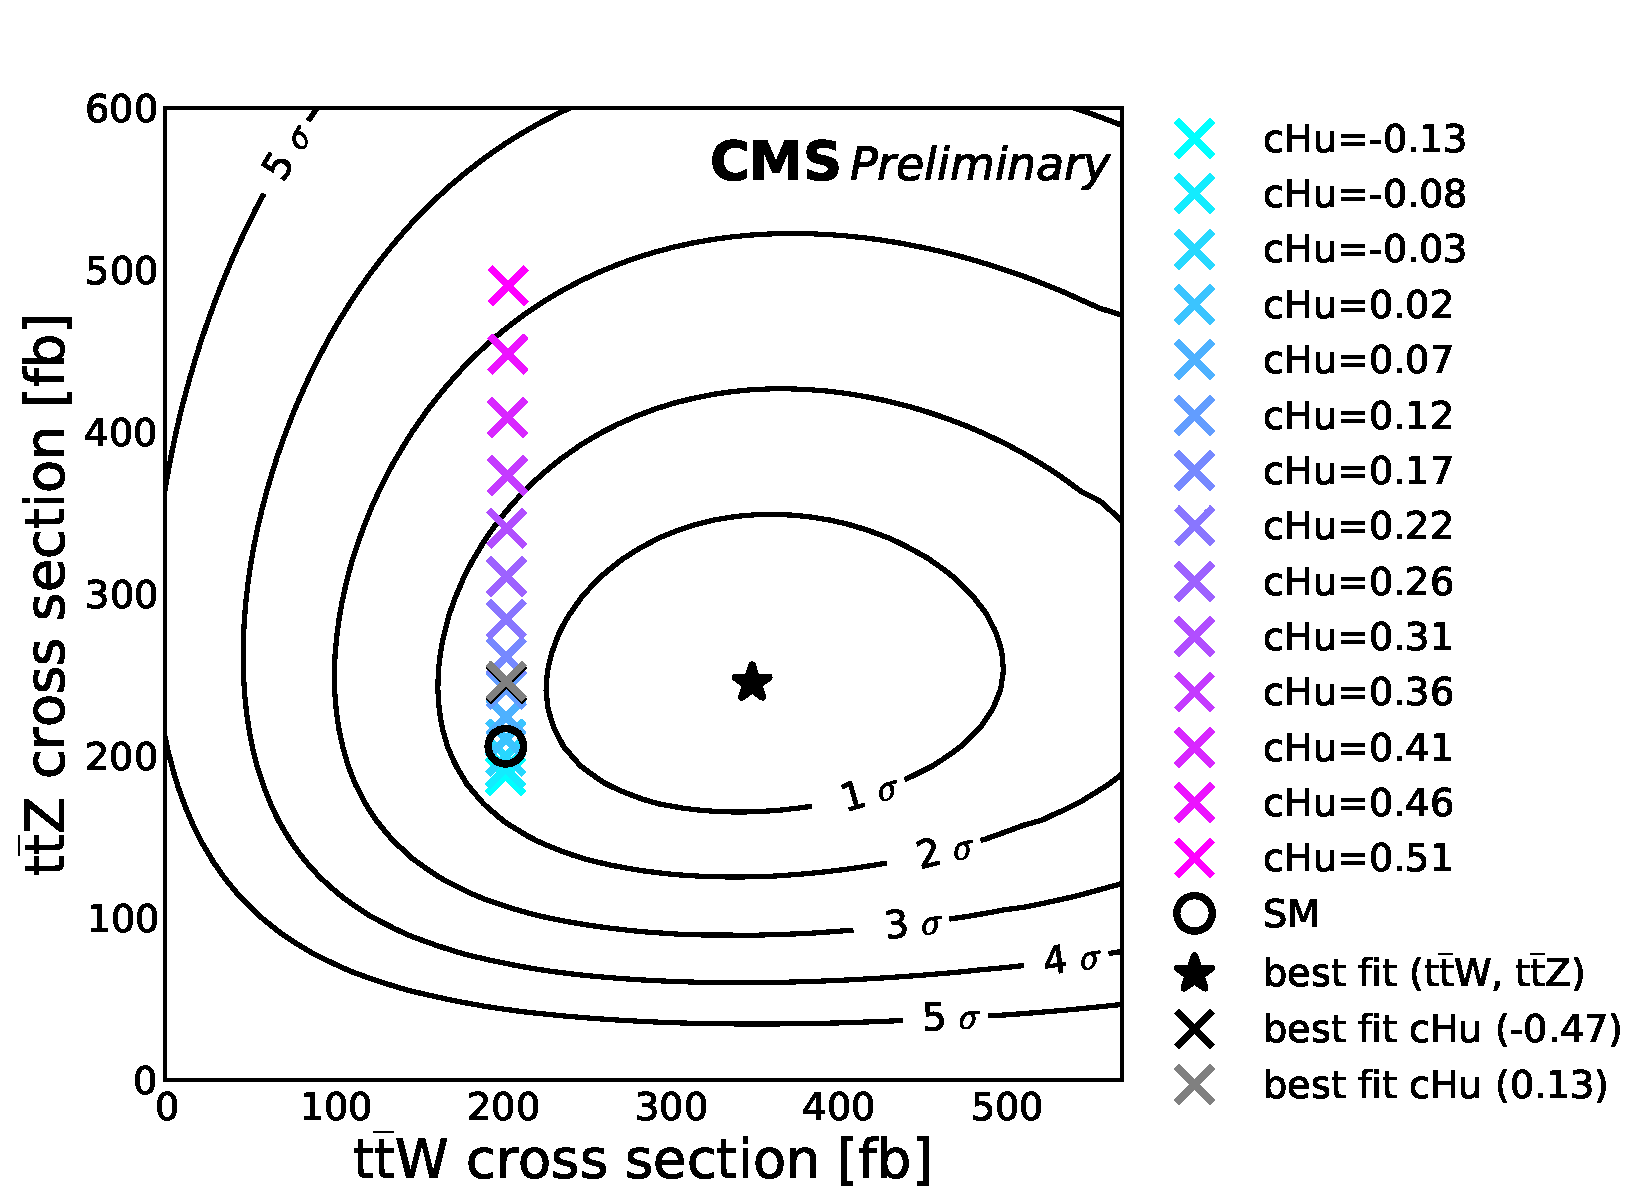
\includegraphics[width=.45\textwidth]{figures/CMS-TOP-14-021_operator_points_color_cycled_cHu_ttZ_ttW_2d_v4}
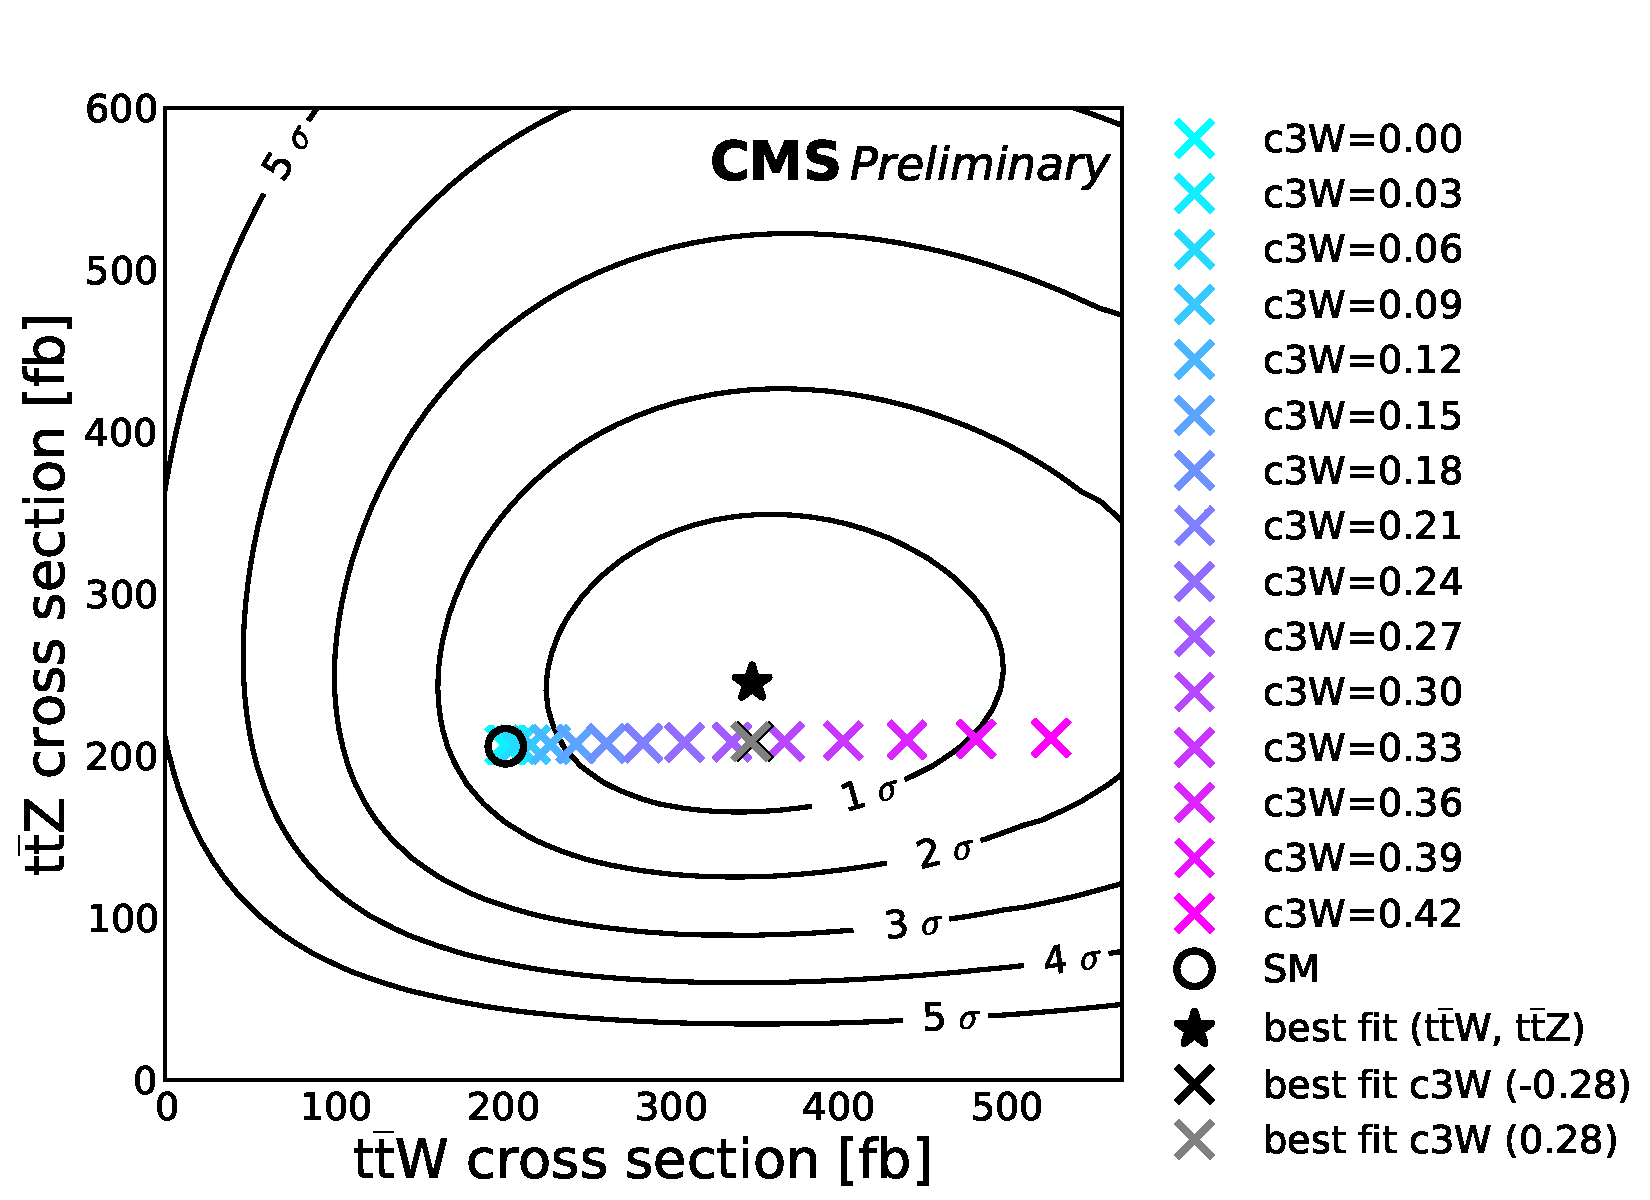
\includegraphics[width=.45\textwidth]{figures/CMS-TOP-14-021_operator_points_color_cycled_c3W_ttZ_ttW_2d_v4}
\caption{Sampled coefficient values for ${\bar c}_{Hu}$ (left) and
  ${\bar c}_{3W}$ (right), plotted in the $\sigma({\rm t{\bar t}W})$,
  $\sigma({\rm t{\bar t}Z})$ plane. There are typically two best fit values, one
  greater and one less than zero, which lie on top of one another in the plane.}
\label{fig:CMS-TOP-14-021}
\end{figure}


%~~~~~~~~~~~~~~~~~~~~~~~~~~~~~~~~~~~~~~~~~~~~~~~~~~~~~~~~~~~~~~~~~~~~~~~~~~~~~~~
\section{Measurement of the ratio $B({\rm t}\to{\rm Wb})/B({\rm t}\to{\rm Wq})$
in pp collisions at $\sqrt{s} = 8~\rm{TeV}$}
%~~~~~~~~~~~~~~~~~~~~~~~~~~~~~~~~~~~~~~~~~~~~~~~~~~~~~~~~~~~~~~~~~~~~~~~~~~~~~~~

The magnitude of the top-bottom charged current is proportional to $|V_{\rm tb}|$,
an element of the Cabibbo-Kobayashi-Maskawa (CKM) matrix. It is expected to be close
to unity and dominate over the off-diagonal elements. Thus, the decay modes of the
top quark to lighter down-type quarks (d or s) are allowed, but highly suppressed.
The indirect measurement of $|V_{\rm tb}|$, from the unitarity constraint of the CKM
matrix, is $|V_{\rm tb}| = 0.999146_{-0.000046}^{+0.000021}$. Any deviation from this value
or in the partial decay width of the top quark to b quarks, would indicate new physics
contributions such as those from new heavy up- and/or down-type quarks or a charged
Higgs boson, amongst others. Here~\cite{CMS_tWb_tWq_ratio} we present a measurement
of $R = B({\rm \to Wb})/B({\rm t \to Wq})$, where the denominator includes the sum over
the branching fractions of the top quark to a W boson and a down-type quark (q = b, s, d).
Under the assumption of the unitarity of the $3 \times 3$ CKM matrix, $R = |V_{\rm tb}|^2$,
and thus to indirectly measure $|V_{\rm tb}|$. In addition, the combination of a
determination of $R$ and a measurement of the t-channel single-top cross section
can provide an indirect measurement of the top quark width $\Gamma_{\rm t}$.

The event selection is optimised for tt dilepton final states that contain two isolated
oppositely charged leptons, missing transverse energy, and at least two jets. The selected
events are categorised by the dilepton channel and the number of observed jets. The
tt dilepton signal strength, $\mu$, defined as the ratio of the observed to the expected
signal rate, is measured from the jet multiplicity distribution by using a profile
likelihood method. A fit including all categories gives the range
$0.909 < \mu < 1.043$ at the 68\% confidence level (CL).

The b flavour content of the selected events (both signal and background) is determined
from the b tagged jet multiplicity distribution. Fig.~\ref{fig:CMS-TOP-12-035} (left)
shows the number of b tagged jets in the selected dilepton data sample, compared to the
expectations from simulation. The multiplicity is shown separately for each dilepton
channel and jet multiplicity. The expected event yields are corrected after the
fit for the signal strength. For a given number of correctly reconstructed and selected
jets, the expected b tagged jet multiplicity can be modelled as a function of $R$ and
the b tagging and misidentification efficiencies. In the parameterisation, we distinguish
events containing jets from 0, 1, or 2 top quark decays.
Fig.~\ref{fig:CMS-TOP-12-035} (right) shows the results obtained
by maximising the profile likelihood. The combined measurement of $R$ gives
$R = 1.014 \pm 0.003~({\rm stat.}) \pm 0.032~({\rm syst.})$, in good agreement with the
SM prediction. The largest contribution to the systematic uncertainty is from the b-tagging
efficiency measurement.

A lower limit of $R > 0.955$ at 95\% CL is obtained after requiring $R \leq 1$ and taking
into account both statistical and systematical uncertainties. This result translates
into a lower limit $|V_{\rm tb}| > 0.975$ at 95\% CL when assuming the unitarity of the
three-generation CKM matrix. By combining this result with a previous CMS measurement of
the t-channel production cross section for single top quarks, an indirect measurement of
the top quark total decay width
$\Gamma_{\rm t} = 1.36 \pm 0.02~({\rm stat.})^{+0.14}_{-0.11}~({\rm syst.})$~GeV is obtained,
in agreement with the SM expectation. These measurements of $R$ and $\Gamma_{\rm t}$ are
the most precise to date and the first obtained at the LHC.


\begin{figure}
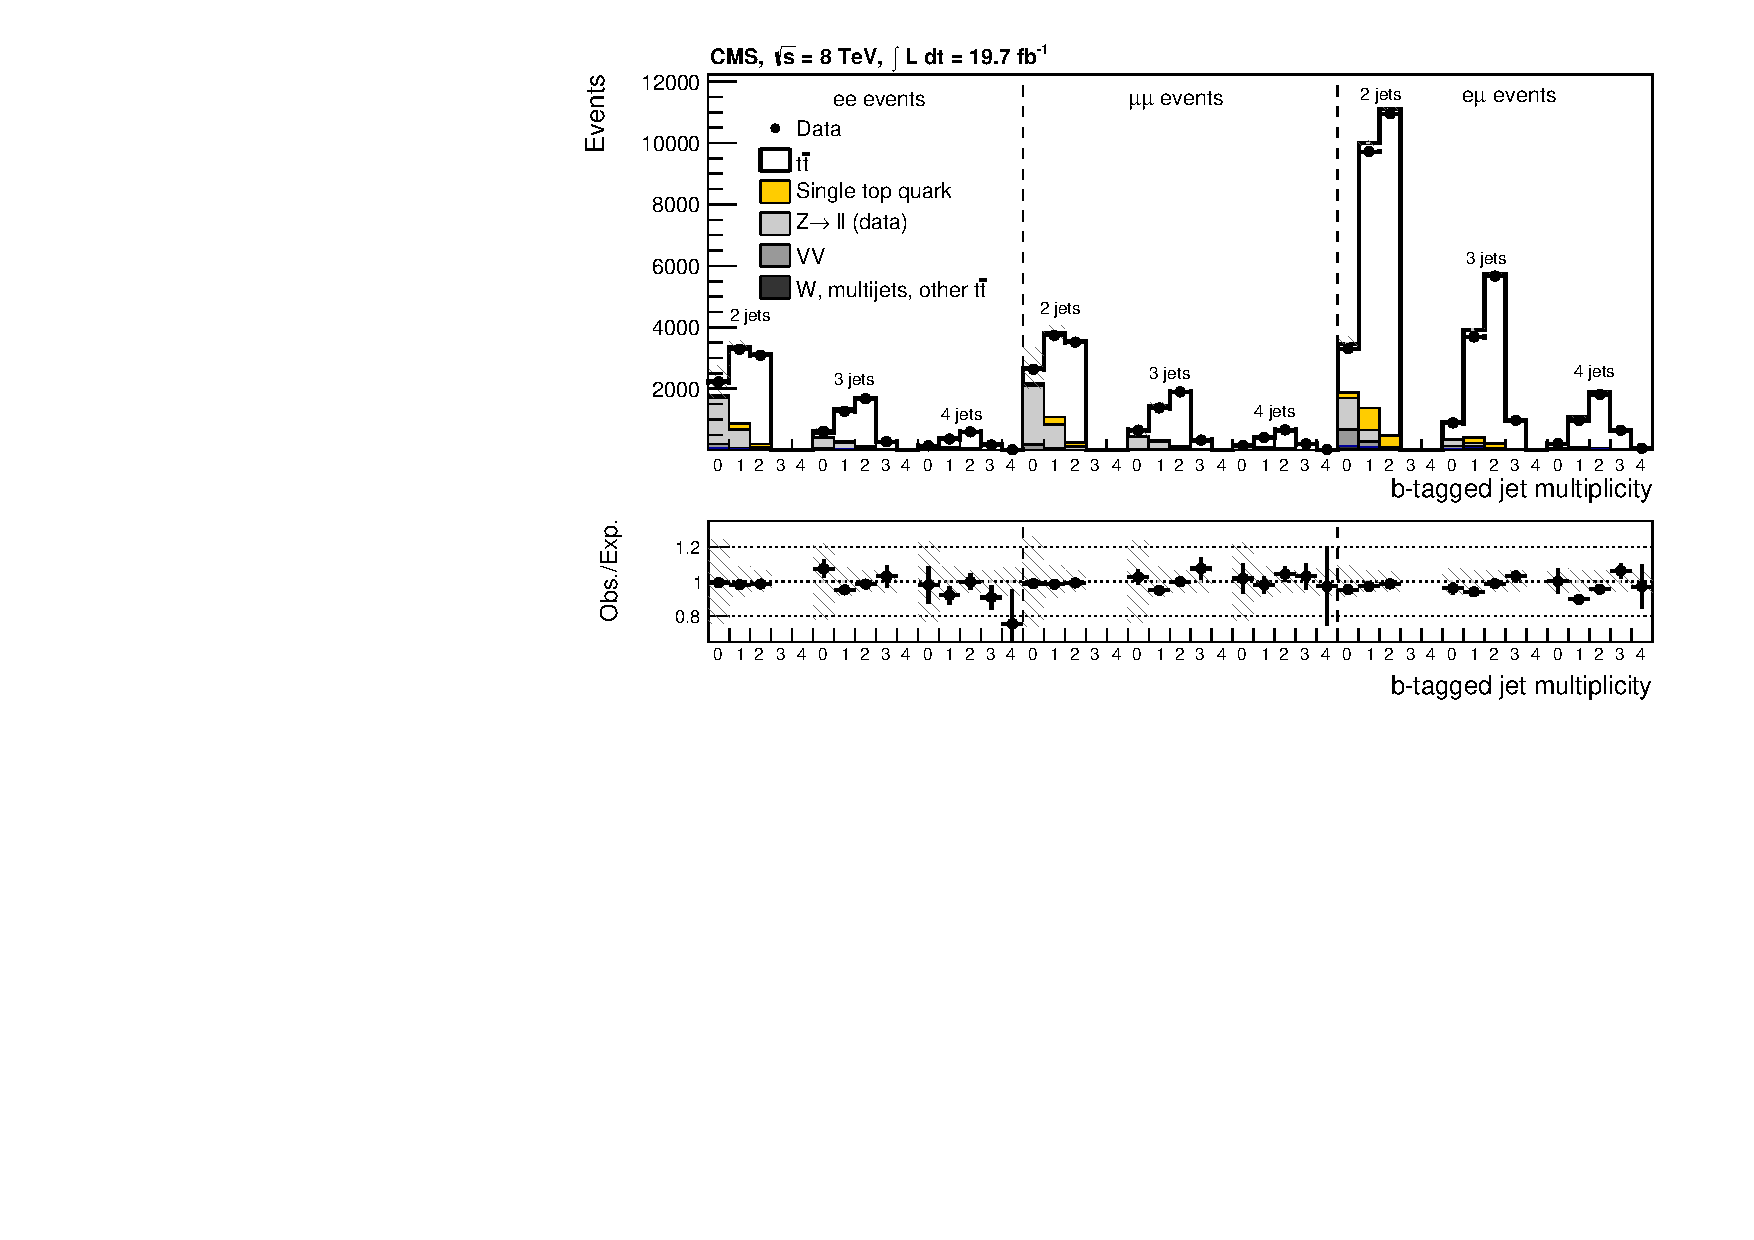
\includegraphics[width=.57\textwidth]{figures/CMS-TOP-12-035_Figure_002}
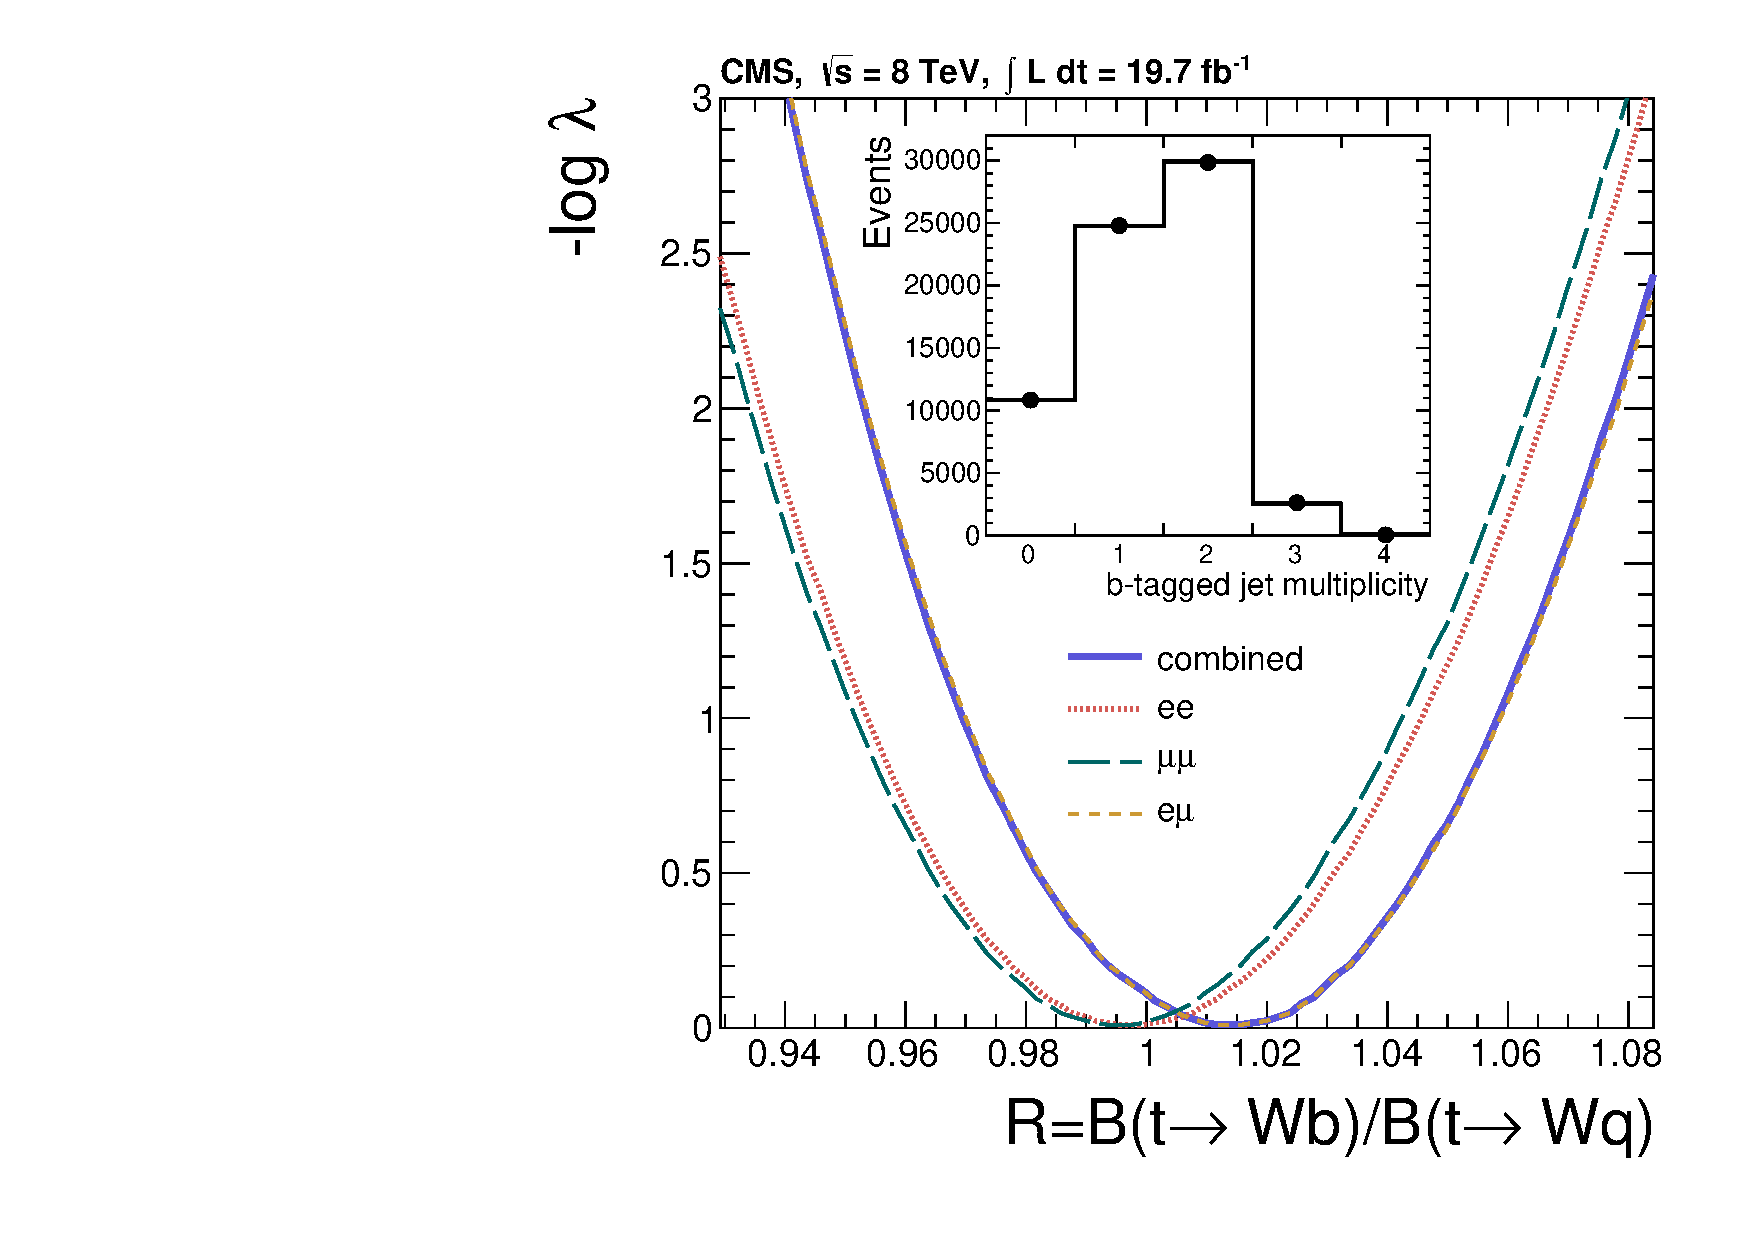
\includegraphics[width=.33\textwidth]{figures/CMS-TOP-12-035_Figure_006}
\caption{(Left) Number of b tagged jets per event for the different dilepton
  channels. For each final state, separate subsets are shown corresponding to
  events with two, three, or four jets. (Right) Variation of the log of the
  profile likelihood ratio used to extract $R$ from the data. The variations
  observed in the combined fit and in the exclusive ee, $\mu\mu$, and e$\mu$
  channels, are shown. The inset shows the inclusive b tagged jet multiplicity
  distribution and the fit distribution.}
\label{fig:CMS-TOP-12-035}
\end{figure}


%~~~~~~~~~~~~~~~~~~~~~~~~~~~~~~~~~~~~~~~~~~~~~~~~~~~~~~~~~~~~~~~~~~~~~~~~~~~~~~~
\begin{thebibliography}{99}
%~~~~~~~~~~~~~~~~~~~~~~~~~~~~~~~~~~~~~~~~~~~~~~~~~~~~~~~~~~~~~~~~~~~~~~~~~~~~~~~

\bibitem{cms}{CMS Collaboration, JINST {\bf 3}, S08004 (2008).}

% W polarization
%~~~~~~~~~~~~~~~~~~~~~~~~~~~~~~~~~~~~~~~~~~~~~~~~~~~~~~~~~~~~~~~~~~~~~~~~~~~~~~~

\bibitem{Wtb}{J.~A.~Aguilar-Saavedra et al.,``Probing anomalous Wtb couplings in
  top pair decays``, Eur. Phys. J. C {\bf 50} (2007) 519-533,
  {\tt doi:10.1140/epjc/s10052-007-0289-4}.}

\bibitem{nnlo-helicity}{A.~Czarnecki, J.~G.~Korner, and J.~H.~Piclum, ``Helicity
  fractions of W bosons from top quark decays at NNLO in QCD``, Phys. Rev. D
  {\bf 81} (2010) 111503, {\tt doi:10.1103/PhysRevD.81.111503}.}

\bibitem{theta-parametrization}{R.~Dalitz and G.~R.~Goldstein,``Decay and
  polarization properties of the top quark``, Phys. Rev. D {\bf 45} (1992) 1531,
  {\tt doi:10.1103/PhysRevD.45.1531}.}

\bibitem{TOP-14-017}{CMS Collaboration, ``Measurement of the W boson helicity
  using ttbar events in the dilepton final state at $\sqrt{s} = 8~{\rm TeV}$``,
  CMS Physics Analysis Summary CMS-PAS-TOP-14-017, 2015.}

\bibitem{semileptonic-helicity-1}{CMS Collaboration, ``Measurement of the W-boson
  helicity in top-quark decays from tt production in lepton+jets events in pp
  collisions at $\sqrt{s} = 7~{\rm TeV}$``, JHEP 10 (2013) {\bf 167},
  {\tt doi:10.1007/JHEP10(2013)167}.}

\bibitem{semileptonic-helicity-2}{CMS Collaboration, ``Measurement of the W-boson
  helicity in top decays from tt production in lepton+jets events at the LHC at
  $\sqrt{s} = 8~{\rm TeV}$``, CMS Physics Analysis Summary CMS-PAS-TOP-13-008,
  2013.}

\bibitem{dileptonic-helicity}{CMS Collaboration, ``Measurement of W-polarization
  in dileptonic tt events in pp collisions with $\sqrt{s} = 7~{\rm TeV}$``,
  CMS Physics Analysis Summary CMS-PAS-TOP-12-015, 2012.}

\bibitem{single-top-helicity}{CMS Collaboration, ``Measurement of the W boson
  helicity in events with a single reconstructed top quark in pp collisions at
  $\sqrt{s} = 8~{\rm TeV}$``, JHEP 01 (2015) {\bf 053},
  {\tt doi:10.1007/JHEP01(2015)053}.}


% Top quark couplings
%~~~~~~~~~~~~~~~~~~~~~~~~~~~~~~~~~~~~~~~~~~~~~~~~~~~~~~~~~~~~~~~~~~~~~~~~~~~~~~~

\bibitem{CMS_tZq_8TeV}{CMS Collaboration, ``Search for Flavor-Changing Neutral
  Currents in Top-Quark Decays ${\rm t \to Zq}$ in pp Collisions at
  $\sqrt{s} = 8~{\rm TeV}$``, PRL {\bf 112}, 171802 (2014).}


% ttV
%~~~~~~~~~~~~~~~~~~~~~~~~~~~~~~~~~~~~~~~~~~~~~~~~~~~~~~~~~~~~~~~~~~~~~~~~~~~~~~~

\bibitem{TOP-14-021}{CMS Collaboration, ``Measurement of top quark pairs produced
  in association with a W or Z boson in pp collisions at $\sqrt{s} = 8~{\rm TeV}$
  using event reconstruction techniques``,
  CMS Physics Analysis Summary CMS-PAS-TOP-14-017, 2015.}


% R=BR(t->Wb)/BR(t->Wq)
%~~~~~~~~~~~~~~~~~~~~~~~~~~~~~~~~~~~~~~~~~~~~~~~~~~~~~~~~~~~~~~~~~~~~~~~~~~~~~~~

\bibitem{CMS_tWb_tWq_ratio}{CMS Collaboration, ``Measurement of the ratio
  $B({\rm \to Wb})/B({\rm t \to Wq})$ in pp collisions at $\sqrt{s} = 8$~TeV``,
  Physics Letter B {\bf 736} (2014) 33-57.}

\end{thebibliography}

\end{document}
